\subsection{Введение}
	Камеры были изобретены и используются уже достаточно долгое время. Однако, с разработкой дешевых камер-обскур в конце 20-го века, камеры стали обычным явлением в нашей повседневной жизни. К сожалению, достижение дешевизны камер имеет свою цену: значительные искажения изображения реального мира. К счастью, получаемые искажения связаны с некоторыми константными (постоянными) значениями, и при помощи калибровки и преобразований можно исправить получаемые изображения. Кроме того, при калибровке вы также можете определить связь между естественными единицами измерения камеры - пикселями, и единицами измерения реального мира, например, миллиметрами.

\subsection{Внутренние параметры}
	Внутренними параметрами камеры являются фокусные расстояния и координаты центра изображения, а точнее, его смещения, т.к. у реальных камер пикселы незначительно, но отличаются от квадратных, а центр имеет ненулевые координаты. Таким образом, внутренние параметры камеры можно представить матрицей \textbf{K}:

	\[
		K = 
		\begin{pmatrix}
			\alpha _x & 0         & x_0 \\
			0         & \alpha _y & y_0 \\
			0         & 0 		  & 1   \\
		\end{pmatrix}
	\]
	
\subsection{Коэффициенты дисторсии}
	Помимо этого, в силу неидеальности оптики, на изображениях, полученных с камер, присутствуют искажения-дисторсии. Они бывают двух видов:
	\begin{itemize}
		\item \textbf{Радиальная дисторсия} - скажение изображения в результате неидеальности параболической формы линзы. Искажения, вызванные радиальной дисторсией, равны 0 в оптическом центре сенсора и возрастают к краям. Как правило, радиальная дисторсия вносит наибольший вклад в искажение изображения.
		
		\item \textbf{Тангенциальная дисторсия} - искажения изображения, вызванные погрешностями в установки линзы параллельно плоскости изображения.
	\end{itemize}
	
	Для устранения дисторсии координаты пикселей можно пересчитать с помощью следующего уравнения:
	
	\begin{gather*}
		u_{corrected} = u(1 + k_1 r^2 + k_2 r^4 + k_3 r^6) + 2 p_1 u v + p_2 (r^2 + 2 u^2) , \\
		v_{corrected} = v(1 + k_1 r^2 + k_2 r^4 + k_3 r^6) + p_1 (r^2 + 2 v^2) + 2 p_2 u v ,
	\end{gather*}
	
	где: 
	\begin{itemize}
		\renewcommand{\labelitemi}{--}
		\item $(u, v)$ - первоначальное расположение пикселя;
		\item $(u_{corrected}, v_{corrected})$ - расположение пикселя после устранения геометрических искажений;
		\item $k1, k2, k3$ - коэффициенты радиальной дисторсии;
		\item $p1, p2$ - коэффициенты тангенциальной дисторсии;
		\item $r^2 = u^2 + v^2$.
	\end{itemize}

\subsection{Исходные данные}
	Для выполнения работы был выслан набор снимков с шахматной доской (15 штук) снятой в разных положениях. Пример показан на рисунке \ref{img:img_example}.
	
	\begin{figure}[h]
		\center{
			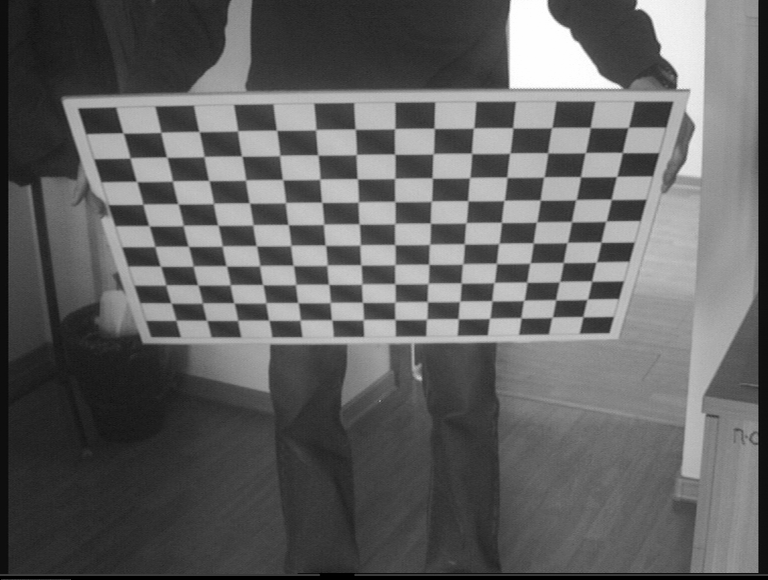
\includegraphics[width=5cm]{img/img_example1.png} \hspace{5mm}
			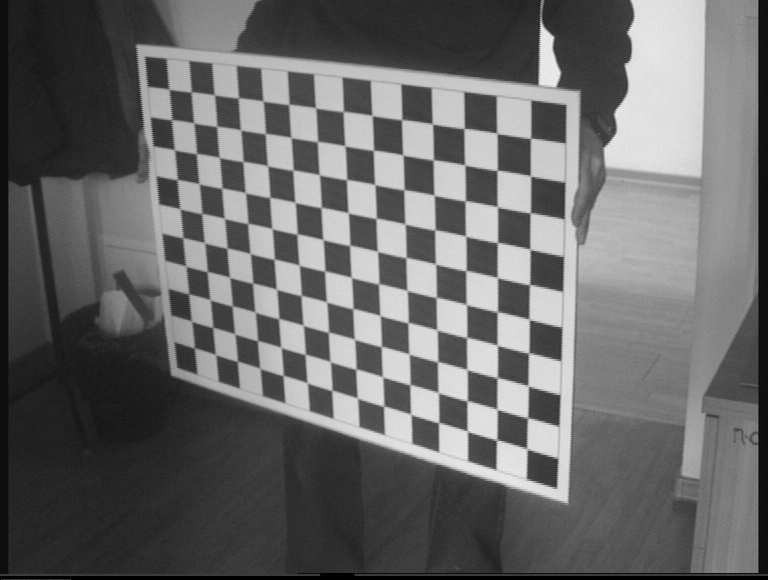
\includegraphics[width=5cm]{img/img_example2.png} \hspace{5mm}
			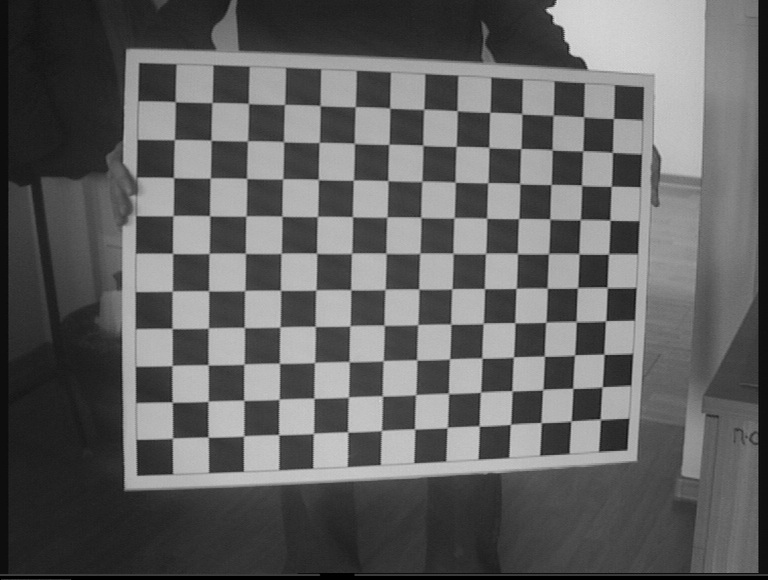
\includegraphics[width=5cm]{img/img_example3.png} \\ \vspace{5mm}
			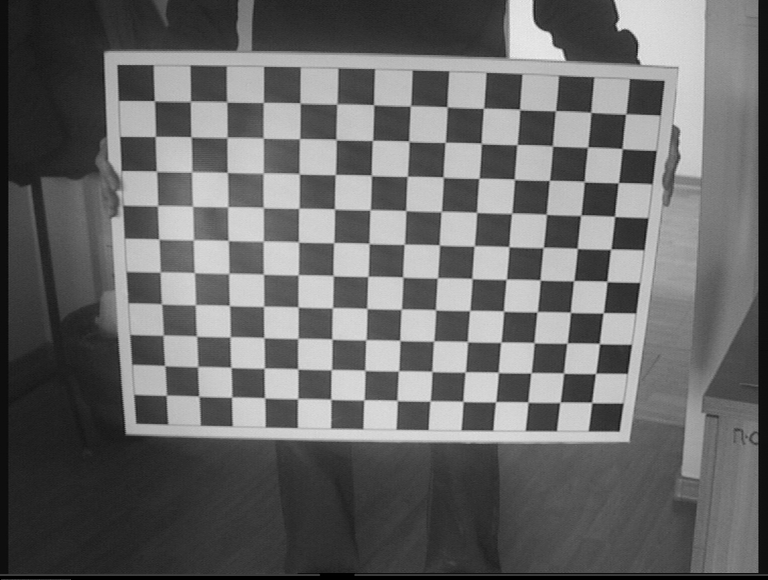
\includegraphics[width=5cm]{img/img_example4.png} \hspace{5mm}
			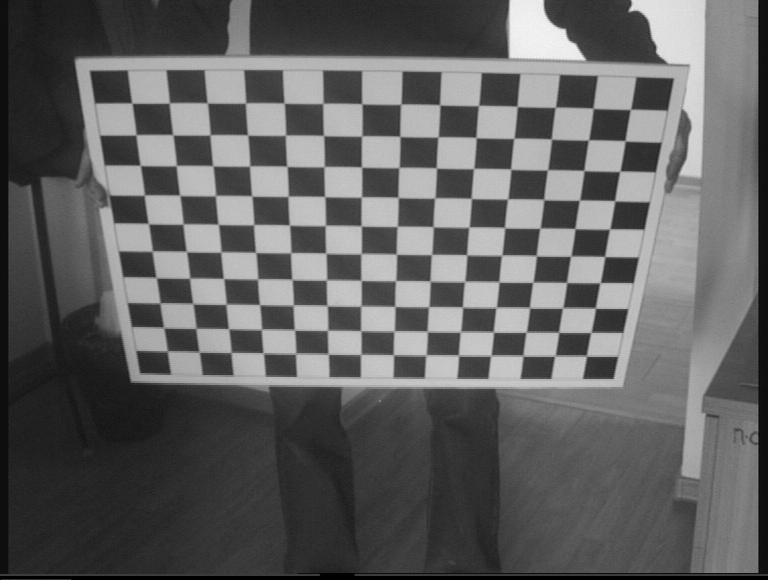
\includegraphics[width=5cm]{img/img_example5.png} \hspace{5mm}
			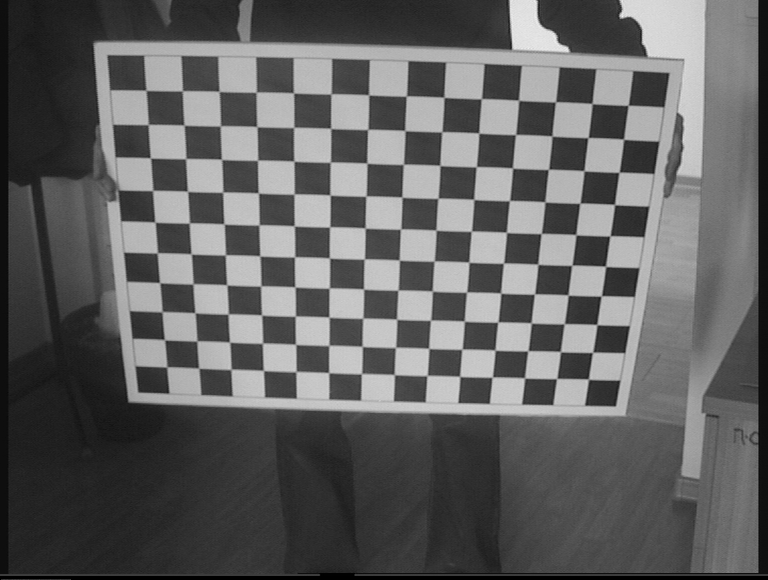
\includegraphics[width=5cm]{img/img_example6.png} \hspace{5mm}
		}
		\caption{Пример фотографий для калибровки.}
		\label{img:img_example}
	\end{figure}

	Кроме того, для сравнения результата, имеются точные данные камеры, на которую снимался этот набор фотографий и по которым мы должны эмпирически получить параметры. $K_{ideal}$ и $C_{distorceIdeal}$ представлены в выражениях \eqref{eq:k_ideal} и \eqref{eq:c_distorce_ideal}.
	
	\begin{equation}\label{eq:k_ideal}
		K_{ideal} = 
		\begin{pmatrix}
			1192.837 & 0 		& 370.637 \\
			0		 & 1192.837 & 304.191 \\ 
			0		 & 0		& 1 
		\end{pmatrix}
	\end{equation}
	\begin{equation}\label{eq:c_distorce_ideal}
		C_{distorceIdeal} = 
		\left[
			\begin{array}{ccccc}
				-0.3470 & 2.223 & 0 & 0 & -12.066
			\end{array}
		\right]
	\end{equation}
			